% Evidence snapshot: repository HEAD 589cf4c, 14 October 2026.
% Baseline attribution: applications/rhoFixedFlowFoam/doc/phase-change-plan.md section 31.
% Wall definitions: manuscript/sections/03-model.tex; solvePairedGasSpecies.H.
% Results: manuscript/generated/{numbers,numerical-table,lobresco-table,alignment-table}.tex.
% Interpretation: manuscript/sections/{06-validation,07-multispecies,08-conclusions}.tex.
% Exactly 10 physical slides. No new CFD runs; saved completed evidence only.
\PassOptionsToPackage{table}{xcolor}
\documentclass[aspectratio=169,9pt]{beamer}
\usetheme{PSI}
\usepackage{amsmath,amssymb,array}
\usefonttheme{professionalfonts}
\ifXeTeX\setsansfont{DejaVu Sans}\fi
\graphicspath{{figures/}{../../manuscript/figures/}{psi-assets/}}
\colorlet{PSIaccent}{PSIyellow}
\colorlet{PSIpale}{PSIyellow!28}
\setbeamercolor{structure}{fg=PSIblack}
\setbeamercolor{itemize item}{fg=PSIblack}
\setbeamercolor{block title}{fg=PSIblack,bg=PSIyellow}
\setbeamercolor{block body}{fg=PSIblack,bg=PSIyellow!14}
\renewcommand{\PSItableheadfg}{PSIblack}
\renewcommand{\PSIfootername}{PSI \textperiodcentered\ LESTO \textperiodcentered\ Group meeting}
\renewcommand{\PSIfootdate}{15.10.2026}
\AtBeginSection[]{}
\AtBeginEnvironment{itemize}{\setlength{\itemsep}{4pt}}
\newcommand{\takeaway}[1]{{\setlength{\fboxsep}{4pt}\noindent\colorbox{PSIyellow}{\parbox{\dimexpr\textwidth-2\fboxsep\relax}{\small\bfseries\strut #1\strut}}}\par\vspace{0.8em}}
\newcommand{\src}[1]{\par\vfill{\scriptsize\color{PSIgray}#1\par}}
\newcommand{\tile}[3]{\colorbox{PSIpale}{\begin{minipage}[t][1.65cm][t]{0.295\textwidth}\vspace{5pt}\raggedright\hspace{5pt}{\fontsize{22}{25}\selectfont\bfseries #1}\par\vspace{3pt}\hspace{5pt}\textbf{#2}\par\hspace{5pt}{\scriptsize #3}\end{minipage}}}
\newcommand{\bigfig}[1]{\includegraphics[width=\linewidth,height=0.57\textheight,keepaspectratio]{#1}}
\begin{document}

% 1
{\setbeamertemplate{footline}{}
\begin{frame}[plain]
\begin{tikzpicture}[remember picture,overlay]
\fill[PSIyellow] (current page.south west) rectangle (current page.north east);
\node[anchor=north west] at ([xshift=0.85cm,yshift=-0.55cm]current page.north west) {
\includegraphics[width=3.4cm]{psi-full-black}};
\node[anchor=west,text width=9cm] at ([xshift=0.95cm,yshift=0.4cm]current page.west) {\small GROUP MEETING\par\vspace{0.4cm}{\fontsize{27}{31}\selectfont\bfseries LESTO project update}\par\vspace{0.3cm}{\large From Bojan's baseline to\\conservative Pb--Bi--I deposition}};
\node[anchor=south west,align=left] at ([xshift=0.95cm,yshift=0.65cm]current page.south west) {\textbf{Jan Kren}\\Paul Scherrer Institute\quad$|$\quad15 October 2026};
\node[anchor=east,fill=white,inner sep=9pt] at ([xshift=-0.8cm,yshift=-0.05cm]current page.east) {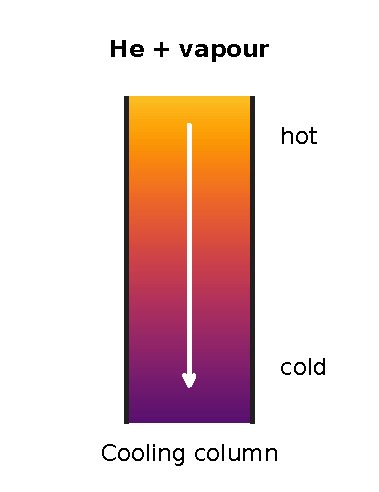
\includegraphics[width=4.0cm]{title-column.pdf}};
\end{tikzpicture}
\end{frame}}

% 2
\begin{frame}[t]{Project status}
\takeaway{The coupled model is implemented; predictive validation remains open.}
\tile{9}{Reactive gases}{Pb--Bi--I; helium carrier}\hfill\tile{4}{Wall inventories}{PbI$_2$, BiI$_3$, Pb, Bi}\hfill\tile{19}{Production reruns}{All pass numerical gates}
\vspace{0.35cm}
\tile{64}{Follow-up cases}{Completed input sensitivities}\hfill\tile{41,472}{Production cells}{Bounded limited-linear advection}\hfill\tile{18 K}{Onset RMS error}{5 independent PbI$_2$ experiments}
\src{Snapshot: 14 October 2026. Production = 15 baseline cases + 4 silica mappings; 64 follow-ups use the earlier upwind mesh.}
\end{frame}

% 3
\begin{frame}[t]{Bojan's baseline}
\takeaway{I retained the conservative mock and added a separate physical phase-change path.}
\psitablecolors{PSIyellow}
\begin{tabular}{p{0.22\linewidth}p{0.33\linewidth}p{0.35\linewidth}}
\rowcolor{PSIyellow}\psihead{Component}&\psihead{Bojan's foundation}&\psihead{My additions}\\
Transport & Frozen-flow species solver & Paired gas--wall exchange\\
Phase change & PbI$_2$ gas-to-solid mock & Reversible, inventory-limited HKS law\\
Conservation & Realised gas sink feeds solid & Gas, wall and Pb/Bi/I element ledgers\\
Thermochemistry & xGEMS probe / startup demo & Optional GEMS bridge + gas equilibrium\\
Evidence & Evolutionary pipe-flow cases & Regression, refinement, experiments\\
\end{tabular}
\vspace{0.2cm}\small Mock path preserved; physical runs use the specialised gas kernel.
\src{Attribution: phase-change plan, section 31; baseline tag 0.1 (7155e6b), integrated main 71bf192.}
\end{frame}

% 4
\begin{frame}[t]{Reversible wall exchange}
\takeaway{Wall kinetics and radial diffusion now share one conservative exchange flux.}
\begin{columns}[c,onlytextwidth]
\begin{column}{0.57\textwidth}
\centering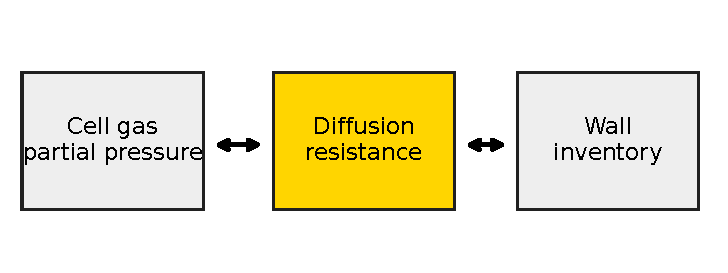
\includegraphics[width=0.90\linewidth]{wall-law.pdf}
\[j_i=G_i^{\rm eff}\,[p_{{\rm eq},i}(T_w)-p_{i,c}]\]
\[\frac{1}{G_i^{\rm eff}}=\underbrace{\frac{1}{G_i}}_{\text{kinetics}}+\underbrace{\frac{\chi_i d_f}{(\rho D_i)_f}}_{\text{half-cell diffusion}}\]
\end{column}
\begin{column}{0.38\textwidth}\begin{itemize}
\item Deposition and re-evaporation
\item No evaporation from an empty store
\item Equal-and-opposite gas/wall transfer
\end{itemize}\vspace{0.25cm}\small No prescribed deposition temperature in the HKS model.
\end{column}\end{columns}
\src{$j_i>0$: wall to gas; $\chi_i=\rho RT/M_i$; $d_f$: cell centre to wall. HKS = Hertz--Knudsen--Schrage.}
\end{frame}

% 5
\begin{frame}[t]{Multispecies thermochemistry}
\takeaway{Chemical redistribution now conserves Pb, Bi and I across shared wall stores.}
\begin{columns}[c,onlytextwidth]
\begin{column}{0.57\textwidth}\centering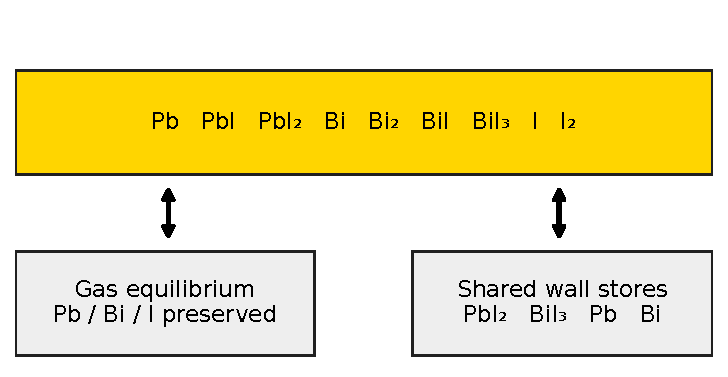
\includegraphics[width=\linewidth]{chemistry.pdf}
\[3\,\mathrm{BiI(g)}\longrightarrow 2\,\mathrm{Bi(cond.)}+\mathrm{BiI_3(g)}\]
\end{column}
\begin{column}{0.38\textwidth}\begin{itemize}
\item 9 gases; 4 condensed inventories
\item Bi and Bi$_2$ share one Bi store
\item Optional frozen/local GEMS modes
\end{itemize}\vspace{0.25cm}\small Reported column runs: ideal-gas kernel.\par\vspace{0.2cm}Frozen helium; no thermal feedback.
\end{column}\end{columns}
\src{Implemented reactive channel is irreversible; equilibrium is a model assumption, not measured reaction kinetics.}
\end{frame}

% 6
\begin{frame}[t]{Numerical verification}
\takeaway{Spatial transport error mattered more than time step or corrector count.}
\begin{columns}[c,onlytextwidth]
\begin{column}{0.59\textwidth}\bigfig{numerics.pdf}\end{column}
\begin{column}{0.37\textwidth}\begin{itemize}
\item 41,472 cells; limitedLinear
\item Finest mesh change: 1.98\%
\item Raw element residue: $1.41\times10^{-12}$
\end{itemize}\vspace{0.25cm}\small 1.98\% is a successive-mesh difference, not a certified error bound.
\end{column}\end{columns}
\src{Shifted-BiI steel case; $E_{L1}=\sum_b|I_b-I_b^{\rm ref}|/\sum_b I_b^{\rm ref}$. No formal grid-convergence index.}
\end{frame}

% 7
\begin{frame}[t]{Published PbI$_2$ benchmark}
\takeaway{Onset-temperature RMS error is 18 K, compared with 35 K for both published models.}
\begin{columns}[c,onlytextwidth]
\begin{column}{0.60\textwidth}\bigfig{onset-errors.pdf}\end{column}
\begin{column}{0.36\textwidth}\begin{itemize}
\item 5 experiments; no wall-law retuning
\item Deposit peaks 1--4 cm upstream
\item 3/5 errors exceed $\pm15$ K
\end{itemize}\vspace{0.2cm}\small Source mole fraction reaches 0.33--0.36: passive-carrier assumption fails locally.
\end{column}\end{columns}
\src{Lobresco et al. (2026), Table 2; run/035. Comparison to published model results, not a new T-Flows run.}
\end{frame}

% 8
\begin{frame}[t]{Thermodynamic sensitivity}
\takeaway{The BiI thermodynamic assumption can reverse the predicted iodide partition.}
\begin{columns}[c,onlytextwidth]
\begin{column}{0.58\textwidth}\bigfig{partition.pdf}\end{column}
\begin{column}{0.38\textwidth}\begin{itemize}
\item Steel Q2; 1\% metal saturation
\item BiI$_3$ iodine share: 94.58\% to 2.01\%
\item Separation survives refinement
\end{itemize}\vspace{0.2cm}\small $+29$ kJ/mol is a surrogate perturbation, not a measured correction.
\end{column}\end{columns}
\src{$f_{\rm BiI_3}=3N_{\rm BiI_3}/(2N_{\rm PbI_2}+3N_{\rm BiI_3})$: deposited iodides only. Q2 iodine release remains prescribed.}
\end{frame}

% 9
\begin{frame}[t]{Silica temperature registration}
\takeaway{A 4--5 cm temperature-coordinate discrepancy dominates the original silica mismatch.}
\begin{columns}[c,onlytextwidth]
\begin{column}{0.59\textwidth}\bigfig{silica.pdf}\end{column}
\begin{column}{0.37\textwidth}\begin{itemize}
\item Original Q1 peaks: 56 / 63 cm
\item Measured peaks: 51 / 59 cm
\item Shift hypothesis: 51 / 59 cm
\end{itemize}\vspace{0.2cm}\small Both mappings are unconfirmed. Their overlap ranking reverses with the advection scheme.
\end{column}\end{columns}
\src{Liu et al. (2025); Q1 production cases. Shift temperature only; keep measured scan fixed. No CFD-fitted alignment.}
\end{frame}

% 10
\begin{frame}[t]{Next steps}
\takeaway{The method is ready for review; better inputs are needed for predictive validation.}
\begin{columns}[t,onlytextwidth]
\begin{column}{0.53\textwidth}
\begin{block}{Completed}\begin{itemize}
\item Conservative physical extension of the baseline
\item Numerical and input-sensitivity evidence
\item Manuscript and D3.8 draft
\end{itemize}\end{block}
\end{column}
\begin{column}{0.43\textwidth}
\begin{block}{Next evidence}\begin{itemize}
\item Original temperature / scan coordinates
\item Source history and BiI thermodynamics
\item Cooling protocol; broader spatial checks
\end{itemize}\end{block}
\end{column}\end{columns}
\vspace{0.25cm}
\begin{block}{For discussion}Which input uncertainty comes first? What is needed for manuscript sign-off?\end{block}

\end{frame}
\end{document}



